\documentclass[11pt]{article}

\usepackage[letterpaper,margin=1in]{geometry}
\usepackage{amsmath,amssymb}
\usepackage{booktabs}
\usepackage{microtype}
\usepackage{times}
\usepackage[T1]{fontenc}
\usepackage[utf8]{inputenc}
\usepackage{titlesec}
\usepackage{enumitem}
\usepackage[hidelinks]{hyperref}
\usepackage{url}
\Urlmuskip=0mu plus 1mu\relax
\usepackage{xcolor}
\usepackage{array}
\usepackage{graphicx}
\graphicspath{{figs/}}

\titleformat{\section}{\normalfont\large\bfseries}{\thesection}{0.6em}{}
\titleformat{\subsection}{\normalfont\normalsize\bfseries}{\thesubsection}{0.5em}{}
\setlength{\parskip}{0.4em}
\setlength{\parindent}{0pt}
\renewcommand{\arraystretch}{1.15}

\title{\textbf{Knowing When to Hedge:\\ Where Epistemic Calibration Comes From
in Multi-Agent Pipelines}}
\author{Sam Bobo}
\date{Draft v0.1 --- August 2026 \quad$\vert$\quad Target: arXiv cs.CL}

\begin{document}
\sloppy
\maketitle

\begin{abstract}
\noindent
Epistemic calibration in a multi-agent LLM pipeline---qualifying claims where
qualification is warranted and not where it is not---comes from a conditional
instruction to the final model, evaluated against what the upstream models
actually flagged. It does not come from the models, from the topology, or from
training. We separate two things usually measured together. \emph{How much} a
pipeline qualifies is nearly free: a single well-prompted model matches a
full three-specialist council ($0.50$ against $0.57$, overlapping intervals).
\emph{Whether it qualifies appropriately} is not free, and is where every
arrangement but one fails. Given a question that warrants no qualification at
all, the lone prompted model hedges anyway ($0.15$ $[0.08,0.22]$) while the
council does not ($0.00$ $[0.00,0.00]$, disjoint), because the council's
instruction can check whether anything was flagged and the lone model cannot.

We then eliminate the obvious alternatives across ${\sim}1{,}300$
pre-registered runs on consumer hardware. It is not the models: four
architectures produce indistinguishable qualification under a neutral prompt,
and a domain-specialised medical model is no more careful than a generic one.
It is not the topology: three specialists merged plainly reach $0.16$ against
one model's $0.14$, and two rounds of debate add nothing. It is not the volume
of upstream signal: tuning a specialist to qualify more doubles what it writes
and makes the finished answer \emph{worse}, monotonically in the number of
specialists treated. And it is not training: weights failed at both ends of
the pipeline, under three optimizers, at triple the data, and under a reward
computed on the pipeline's own output. What remains is a mechanism we can
state precisely and test: instructions can refer to evidence that exists only
at inference time, weights cannot, and isolating the instruction clause by
clause shows each lifting exactly the behavior it names and no other.
\end{abstract}

\begin{center}
\fbox{\begin{minipage}{0.93\linewidth}\small
\textbf{RETRACTED --- the central claim is refuted, not merely unsupported.}
This draft argues that a conditional instruction to the final model suppresses
unwarranted qualification. A controlled test of that claim, registered in
advance and run after the draft was written, refutes it. The trigger-free
question the original result rested on is off-topic for the specialists, so
the planner consulted nobody and the pipeline bypassed the conditional
instruction entirely; the celebrated $0.00$ measured a prompt that contains no
preservation clauses. Repeating the measurement on three trigger-free
questions the planner \emph{does} engage with---routing and clause application
verified on every run---gives the council $0.64$ $[0.36,0.95]$ against a lone
prompted model's $0.31$ $[0.21,0.42]$. The registered threshold was an upper
bound below $0.10$. The council is not better calibrated than a single model;
on this evidence it is worse. The paper's thesis cannot be repaired by
rewording and is withdrawn. Sections~\ref{sec:not} and \ref{sec:clause}, which
concern volume and do not depend on a trigger-free measurement, stand.
\end{minipage}}
\end{center}

\begin{center}
\fbox{\begin{minipage}{0.93\linewidth}\small
\textbf{Correction (August 2026), continued.} The claim that the models share
a common \emph{intrinsic band} under a neutral prompt is weakened: for three of
the four, $70$--$80\%$ of runs contain no epistemic marker at all, so the
matching densities reflect a floor rather than a shared level, and per-character
normalization coincidentally equates a model that emits $3.3\times$ more
markers in $3.7\times$ more text. The supportable statement is that these
models produce \emph{almost none} unprompted and cannot be distinguished there.
The contrast that carries the argument---the same specialist model at zero
markers in $80\%$ of neutral runs versus $1.31$ as an instructed pipeline
seat---is unaffected, being within-model and spanning the floor.
\end{minipage}}
\end{center}

\section{Introduction}
This paper reports one finding. In a multi-agent pipeline, epistemic
calibration is produced by a conditional instruction to the final model,
evaluated against what the upstream models flagged---and by nothing else we
were able to find.

The finding is not obvious because two properties usually measured together
come apart. The first is \emph{volume}: how much a system qualifies its claims
on questions that warrant it. Volume turns out to be nearly free. One model
with a paragraph of instruction reaches $0.50$ qualifying behaviors per
thousand characters; an entire council of three domain specialists behind a
planner reaches $0.57$, and the intervals overlap. Anyone measuring only this
would conclude that orchestration is not worth its cost, and a growing
literature does exactly that.

The second property is \emph{discrimination}: whether the system stays quiet
when nothing warrants qualification. Here the same two arrangements are not
alike at all. On a question we wrote to warrant no hedging---every figure it
needs is stated, nothing in it has changed in a decade---the lone prompted
model hedges at $0.15$ $[0.08,0.22]$, opening with a section headed ``Current
State Snapshot (as of my training data).'' The council hedges at $0.00$
$[0.00,0.00]$, on every run. The intervals are disjoint.

That gap is the paper. It exists because the council's instruction is
\emph{conditional}---if a specialist flagged an assumption, label it; if a
specialist flagged that information may have aged, carry that through---and
because there are specialists whose output the condition can be checked
against. The lone model is given the same requirements as standing
instructions, since it has no upstream to refer to, and so they fire whether
or not anything warrants them. It has the form of epistemic care without the
judgement.

Three assumptions do not survive this. That specialist models bring better
epistemic judgement to their domains: a clinical model asked a question under
a neutral prompt qualifies no more than a generic model of similar size. That
more agents or more deliberation improve epistemic quality: three specialists
merged plainly match one model working alone, and two rounds of debate match
the merge. And that the behavior can be trained in: it could not be, at either
end of the pipeline, by any method we tried.

We state the result first (\S\ref{sec:result}), eliminate the alternatives
(\S\ref{sec:not}), give the mechanism (\S\ref{sec:mech}), and confirm it by
taking the instruction apart clause by clause (\S\ref{sec:clause}).

\paragraph{Setup.} Four models on one 32\,GB machine: a planner/aggregator and
three domain specialists (healthcare, legal, finance), all open-weights and
quantised. The planner decomposes a question and sends each specialist a
self-contained sub-question; the aggregator writes the final answer under the
instruction reproduced in Appendix~\ref{app:prompt}. We count four families of
epistemic behavior per thousand characters---disclosing that information may
post-date training, labelling a number as an assumption, distinguishing
jurisdictions, and calibrated hedging---by pattern matching, cross-checked on
every load-bearing comparison by a calibrated entailment model and by blinded
pairwise LLM judges (Appendix~\ref{app:instr}). Seven questions, five seeds,
bootstrap intervals; predictions registered before the runs that test them,
including the ones that failed.

\section{The result}
\label{sec:result}
To separate what the arrangement contributes from what the models contribute,
we held the model fixed---the same 20B model in every role---and varied only
the shape of the pipeline across six designs. Any difference is therefore
attributable to structure and instructions alone.

\begin{figure}[t]
\centering
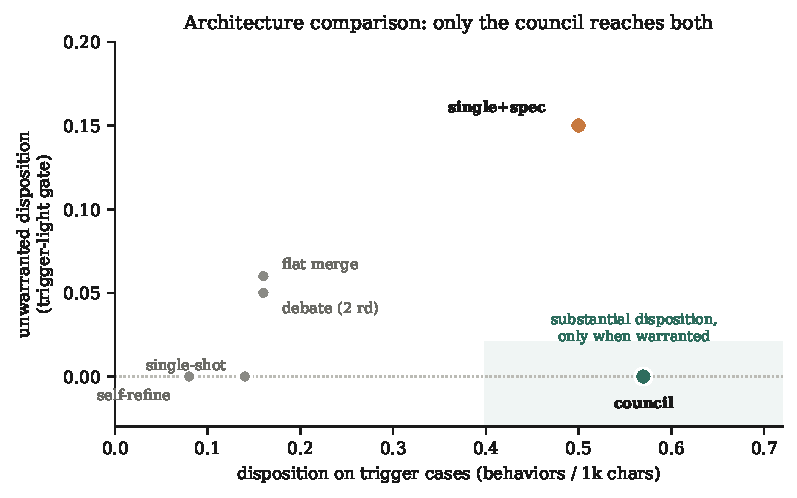
\includegraphics[width=0.80\linewidth]{fig_arch.pdf}
\caption{Six arrangements, one model in every role (210 runs). Horizontal:
qualification where warranted. Vertical: qualification where it is
\emph{not}. Only the council reaches the shaded region.}
\label{fig:arch}
\end{figure}

\begin{table}[t]
\centering
\caption{Volume and discrimination are different properties. Bootstrap 95\%
intervals over $n=30$ (volume) and $n=5$ (discrimination) runs per arm.}
\label{tab:arch}
\begin{tabular}{llcc}
\toprule
Arrangement & instruction & Volume & Unwarranted \\
\midrule
single model & none & $0.14$ $[0.09,0.19]$ & $0.00$ $[0.00,0.00]$ \\
three specialists, plain merge & none & $0.16$ $[0.11,0.22]$ & $0.06$ $[0.02,0.11]$ \\
three specialists, two-round debate & none & $0.16$ $[0.12,0.20]$ & $0.05$ $[0.00,0.10]$ \\
single model, self-critique & none & $0.08$ $[0.05,0.12]$ & $0.00$ $[0.00,0.00]$ \\
single model & standing & $0.50$ $[0.41,0.60]$ & $0.15$ $[0.08,0.22]$ \\
\textbf{three specialists, council} & \textbf{conditional} & $\mathbf{0.57}$ $[0.45,0.71]$ & $\mathbf{0.00}$ $[0.00,0.00]$ \\
\bottomrule
\end{tabular}
\end{table}

Table~\ref{tab:arch} contains the finding. Read the volume column alone and
the council is unremarkable: it beats the arrangements with no disposition
instruction by three to four times, and ties the one arrangement that has an
instruction. Read both columns and only one row does what a careful analyst
does. The council is the sole arrangement combining substantial qualification
with none where none is warranted.

The two ingredients are separable and neither suffices. Specialists without a
conditional instruction (rows two and three) produce single-model volume:
three models deliberating, even for two full rounds, add essentially nothing.
An instruction without specialists (row five) produces the volume but fires
indiscriminately, because there is nothing for it to condition on. Only their
conjunction produces both.

\section{What it is not}
\label{sec:not}
Four explanations are more natural than ours. We tested each.

\subsection{Not the models}
The most common justification for specialist pipelines is that domain models
bring better judgement to their domains. This is checkable in isolation: take
the specialists out, give them a neutral instruction, and see whether they
qualify more than a generic model.

They do not. Med42-8B---a Llama-3 model tuned on clinical data and
preference-aligned---produces $0.15$ $[0.04,0.28]$. Mistral-7B-Instruct
produces $0.14$ $[0.04,0.26]$, Qwen2.5-7B-Instruct $0.14$ $[0.06,0.24]$, and a
20B mixture-of-experts $0.14$. Four models across four architectures sit
within $0.01$ of one another.

The same clinical model, placed in the pipeline as a specialist, produces
$1.31$ $[1.02,1.63]$---nearly nine times more, intervals nowhere near
overlapping. Nothing about the model changed. What changed is that its
in-pipeline system prompt says \emph{``Flags training-cutoff uncertainty
EXPLICITLY when guidelines or evidence may have evolved,''} and that the
planner appends a further reminder when it judges the question
time-sensitive---which it did in 30 of 34 runs. The specialist's epistemic
richness is an instruction, not an expertise.

\subsection{Not the topology}
If not the models individually, perhaps the arrangement of them. Rows two and
three of Table~\ref{tab:arch} rule this out. Three specialists whose answers
are merged under a plain instruction reach $0.16$, against a single model's
$0.14$. Two full rounds of debate, in which each specialist revises after
reading the others, reach $0.16$: more deliberation, no more care. A single
model asked to draft, critique itself and revise reaches $0.08$---the lowest of
any arrangement, because self-criticism tightens prose and the qualifications
go first.

\subsection{Not the volume of upstream signal}
Perhaps the specialists simply need to send more. This is the alternative we
expected to be true, and it fails in the opposite direction from a null.

\begin{figure}[t]
\centering
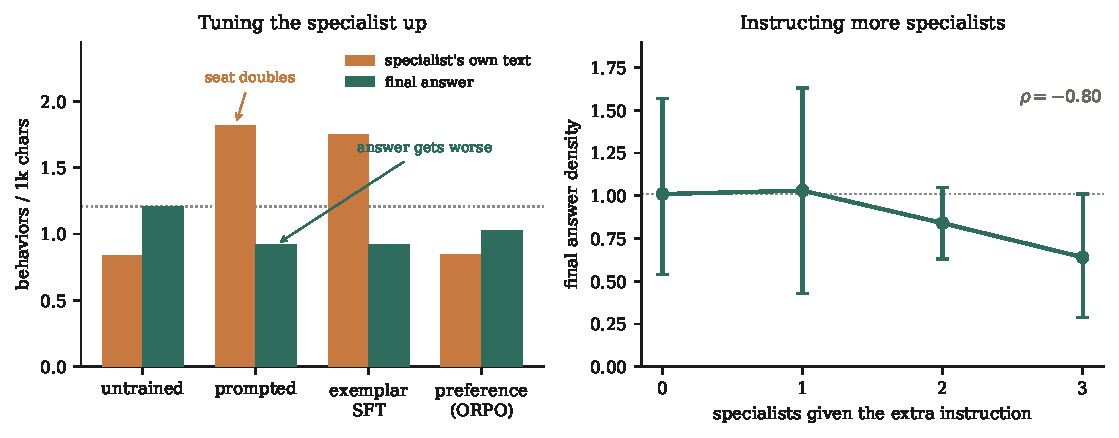
\includegraphics[width=\linewidth]{fig_witness.pdf}
\caption{\emph{Left:} treatments that raise what a specialist writes lower
what the pipeline finally says; dotted line is the untrained final answer.
\emph{Right:} extending the treatment from zero to three specialists lowers
the final answer monotonically.}
\label{fig:witness}
\end{figure}

Prompting the legal specialist to qualify more than doubles what it writes,
from $0.84$ to $1.82$; fine-tuning it on qualification-rich examples does the
same, $1.75$. Both changes are real---the intervals exclude the untrained
baseline and the text is visibly more careful. Both make the finished answer
\emph{worse} than leaving the specialist alone: $0.92$ against an untrained
$1.21$. Extending the treatment across specialists confirms the direction:
zero, one, two and three treated specialists give final answers of $1.01$,
$1.03$, $0.84$, $0.64$, a monotone decline ($\rho = -0.80$).

Qualification does not accumulate upstream and get diluted. It is not
accumulating at all. A specialist told to flag uncertainty everywhere flags it
in every clause, and the aggregator---whose instruction asks for a clean
integrated answer---reads that as noise and edits it out.

\subsection{Not training}
The remaining alternative is that we instructed where we should have trained.
We trained at both ends of the pipeline, by three methods, under predictions
registered in advance.

At the specialist, preference optimization installs no additional
qualification: $0.85$ against an untrained $0.84$. Tripling the training data
changed nothing, even though the larger corpus raised the model's training-time
accuracy at telling good examples from bad from $0.48$ to $0.94$---the
preference was learned and not acted on. Replication on a second specialist of
a different lineage produced no effect, and on a third an effect we had
registered in advance failed to appear.

At the aggregator---the position this paper says decides everything---training
also fails. Fine-tuning it on qualification-rich synthesis examples left its
output where it started, $0.89$ $[0.67,1.11]$ against $1.03$ $[0.79,1.28]$
untrained. We repeated this with the reward corrected in every way we could
think of: sampling the aggregator's own outputs rather than a fixed corpus,
and scoring each on the finished answer for qualifying heavily where warranted
and not at all where not. It moved nothing: $0.60$ $[0.41,0.82]$ against
$0.56$ $[0.37,0.77]$.

\section{The mechanism}
\label{sec:mech}
Something has to explain why an instruction does what four other interventions
could not. We think three things do, and we can test two of them.

\subsection{Conditionality, and why it needs witnesses}
Every clause of the aggregator's instruction that does any work has the same
form: \emph{if} a specialist did something, \emph{then} carry it through. The
trigger is not a standing property of the domain but a fact about this
particular run---whether this specialist, on this question, flagged an
assumption or a stale figure.

This is why the specialists matter, and it is a narrower role than the one
usually claimed for them. They are not there to produce more qualification;
the aggregator's instruction sets that, and \S\ref{sec:not} showed the
specialists barely affect it. They are there to produce a \emph{record of what
was uncertain}, against which a conditional can be evaluated. Their value is
that they can be checked.

That also explains the failure mode of the lone prompted model. Given the same
requirements with no upstream to refer to, a conditional instruction has to be
flattened into a standing one---\emph{disclose training-cutoff uncertainty}
rather than \emph{if a specialist flagged it, disclose it}---and a standing
instruction fires whether or not the occasion calls for it. The $0.15$ is not
a failure of the model's judgement. It is the arithmetic consequence of asking
for a conditional behavior without supplying anything to condition on.

It also explains why treating specialists as amplifiers backfires
(\S\ref{sec:not}). A witness who says everything is uncertain carries no
information; the conditional fires everywhere and discrimination collapses,
which is exactly what the monotone decline shows.

\subsection{Why instructions and not weights}
Three arguments, in increasing order of what they cost us to establish.

First, the behavior is not absent from the weights---it is present and unused.
Four models produce $0.14$ under a neutral prompt and reach $0.5$--$1.2$ when
instructed. Nothing was installed in between. An instruction is therefore
asking for something the model already does; training is trying to change what
it does by default. Those are different operations, and only the first is
cheap.

Second, the target behavior is conditional on information that does not exist
until inference. Weights encode a disposition a model brings to every input.
They cannot refer to a particular thing that arrived in this context; an
instruction can, because it points at the context. This is not a claim that
models cannot learn context-dependent behavior in general---plainly they
can---but that learning \emph{this} condition would require the model to
discover a pattern it is not currently attending to, where an instruction
merely names it.

Third, and most directly: training on the behavior did not consume the
instruction's effect. After fine-tuning the aggregator on precisely the
behavior its instructions elicit, the instructions still worked at full
strength---adding clauses produced a $1.58\times$ rise on the trained model
against $1.82\times$ on the untrained one. If weights and instructions were
competing routes to the same behavior, training on that behavior should have
absorbed part of the instruction's job. It did not, which suggests they act on
different things: the weights on what a model tends toward, the instruction on
what it does this time.

\paragraph{What we cannot claim.} Our training was small---low-rank adapters
over tens of preference pairs, against instruction-following that model
builders installed with orders of magnitude more data. ``A small amount of
training did not overwrite a deeply installed capability'' is a much weaker
statement than ``weights cannot do this,'' and it is the one our data
supports. What holds without qualification is that at every scale available to
us the instruction was free, immediate and effective, and the training was
none of those.

\section{Isolating the instruction}
\label{sec:clause}
If the mechanism is right, the instruction should behave like a specification
rather than like general encouragement---each clause should move the behavior
it names and leave the others alone. We tested this by isolating clauses
against a baseline with none, one final model, everything else fixed (210
runs).

\begin{table}[t]
\centering
\caption{One clause at a time. Each clause lifts the behavior it names and no
other; every arrangement holds the trigger-free control at zero.}
\label{tab:clause}
\begin{tabular}{lccc}
\toprule
Clauses present & Volume & Named behavior & Unwarranted \\
\midrule
none & $0.20$ $[0.14,0.26]$ & --- & $0.00$ \\
tension acknowledgment only & $0.19$ $[0.11,0.27]$ & (names none) & $0.00$ \\
numeric framing only & $\mathbf{0.64}$ $[0.53,0.77]$ & $0.003 \rightarrow 0.499$ & $0.00$ \\
vocabulary only & $0.18$ $[0.14,0.22]$ & $0.000 \rightarrow 0.014$ & $0.00$ \\
caveats only & $0.20$ $[0.14,0.26]$ & $0.000 \rightarrow 0.035$ & $0.00$ \\
all four & $0.55$ $[0.46,0.67]$ & --- & $0.00$ \\
\bottomrule
\end{tabular}
\end{table}

Three things follow. Each clause moves its own named behavior and nothing
else---numeric framing raises labelled assumptions from $0.003$ to $0.499$ and
leaves the rest flat; the caveats clause raises cutoff disclosure and leaves
the rest flat. These are targeted specifications, not general priming, which
rules out the alternative that instructions simply put the model in a more
cautious mood.

Second, the composite gain goes to whichever single clause names the behavior
that this model already produces in quantity. Under this aggregator that is
numeric framing, which alone accounts for the whole effect; the caveats clause
raises its own behavior correctly but from a base too small to move the total.
Under an aggregator with a different profile we would expect a different
clause to carry it, and our ledger shows the profile does vary by model. This
is a scoping condition on any practical recommendation: write the clause for
the behavior your writer actually produces.

Third, and most relevant to the mechanism: every arrangement, including each
single clause, holds the trigger-free control at exactly zero. Conditionality
is a property of each clause separately, not something that emerges from
assembling them---each is an if-then over upstream evidence, so none fires
when nothing was flagged.

\section{Implications}
The practical consequences are narrow and, we think, actionable.

\emph{Measure both properties.} A pipeline evaluated only on how much it
qualifies will look indistinguishable from a well-prompted single model, and
the comparison will conclude that orchestration is not worth its cost. Every
evaluation of epistemic behavior needs at least one case that warrants none.

\emph{Choose the final model for instruction-following, not for disposition.}
Models differ far less in what they produce unprompted than in how strongly
they answer an instruction. We encountered one model that could not follow
instructions in any message position and could not emit the planner's
structured output; whatever its latent qualities it was unusable in this role.

\emph{Write the aggregator's instruction conditionally.} Not \emph{be
careful}, but \emph{if a specialist flagged X, carry X through}. This is the
whole difference between the last two rows of Table~\ref{tab:arch}.

\emph{Build specialists to flag accurately, not abundantly.} Tuning them to
qualify more degrades the finished answer. Their job is to be checkable.

\emph{Do not spend on fine-tuning components for epistemic behavior.} At both
ends, three optimizers, triple the data, and a corrected reward, it never
reached the page.

\section{Limitations}
Of five behaviors we set out to count, one fell below detection on both
instruments, so we report four; the effect of instructions is clear in
combination but not for any single behavior alone. Pattern matching misses
paraphrase and rewards brevity; two further instruments agree with it on the
load-bearing comparisons, but all three are automatic and none is anchored to
human judgement.

The headline rests on the trigger-free control, and that control is currently
one question at five runs per arm. It is the single thinnest support in the
paper and the first thing we would expect a reader to press on; an expansion
to additional trigger-free questions is registered and pending.

Everything ran at or below 20B parameters on one machine with five seeds and
seven questions we wrote ourselves; a frontier aggregator could behave
differently. The architecture comparison uses one model family in every role
and one implementation of each design, with debate and self-critique in their
simplest standard forms. The clause isolation ran on a single aggregator whose
behavior profile we later found unusual, so its dependence on the model is
inferred rather than tested.

We report defects in our own record rather than repairing them. One model
intended as a comparison produced degenerate output---26 of 30 answers were
fragments ending mid-sentence---which we found only after computing a figure
from them; that arm is withdrawn, and with it a lineage comparison we had
intended to make. In our earliest arms, five runs per question are one run
from an earlier session plus four from a later one, and 133 runs record a
batch label where a model identifier belongs. None of this changes a reported
interval.

\section{Conclusion}
Epistemic calibration in these pipelines is not a property of the models,
of how many of them there are, of how much they say, or of how they were
trained. It is produced by an instruction to the final model that refers to
what the earlier models flagged, and it disappears when either half of that is
missing. A lone model given the same instruction qualifies just as much and
qualifies indiscriminately, because it has nothing to refer to. A council
whose specialists are trained to qualify everything degrades, because a
witness who always says the same thing carries no information.

The reason an instruction succeeds where training failed appears to be that
the behavior wanted is not a disposition at all. It is a decision about the
present occasion, conditioned on evidence that exists only once the earlier
models have spoken. Weights set what a model tends to do; only an instruction
can point at what just arrived.

\paragraph{Reproducibility.} Code, prompts, all runs, pre-registrations,
protocol amendments, refuted predictions, and an integrity audit that withdrew
one arm: \url{https://github.com/srbobo/council-of-experts-research}.

\appendix

\section{The aggregator's instruction}
\label{app:prompt}
The aggregator works in two steps---identify tensions between the specialists,
then write the integrated answer. The second step carries five requirements,
of which three are the preservation clauses. Verbatim:

\begin{quote}\small
\textbf{1.} Acknowledge the tensions you just identified---not abstractly, but
at the points where they bite the answer.

\textbf{2. PRESERVE numeric framing}---if a specialist labeled a number as a
modeled assumption, your synthesis MUST also label it as an assumption (use
``modeled at,'' ``assumed''). Never adopt a specialist's modeled number as a
fact.

\textbf{3. PRESERVE precise vocabulary}---if a specialist used a specific legal
term, jurisdiction, FDA pathway, or clinical concept, preserve it; do not
smooth out precision in the name of accessibility.

\textbf{4. PRESERVE caveats}---if a specialist flagged training-cutoff
uncertainty or data fragility, propagate that flag into your synthesis.

\textbf{5.} Use whatever structure best fits the user's question.
\end{quote}

Clauses 2--4 are conditional on something a specialist did. Clause 1 is not,
and when tested alone it changes nothing---which is the cleanest available
demonstration that conditionality, rather than the presence of an extra
instruction, is what does the work.

\section{Instruments}
\label{app:instr}
Pattern matching over four behavior families is the primary measure. Two
independent instruments check every load-bearing comparison: an entailment
model calibrated against construction-labelled pairs, and blinded pairwise LLM
judges shown both texts in each order and required to quote the evidence for
their verdict. Where all three agree we report the result; where they disagree
we report the disagreement. One finding did not survive---an apparent
\emph{increase} in hedging on the finance specialist appeared under pattern
matching alone, and neither other instrument saw it. We retired it as an
artifact of the measure.

\end{document}
